\documentclass[11pt,dvipdfmx]{ujarticle}
\bibliography{3rd_power}
\usepackage{eee}
\usepackage{subfig}

\renewcommand{\labelenumi}{\alph{enumi}}
\renewcommand{\labelenumii}{\roman{enumii}}

\begin{document}

\begin{jikkenTitle}
 \gakunen{3} 
 \numTitle{3}{電力と力率} % 実験番号,タイトルを記述
 \subTitle{} % サブタイトルがあれば記述
 \jikkenbi{令和  年  月  日(  )} % 実験日を記述
 \jikkenbiII{令和  年  月  日(  )} % 実験日を記述(二日目がある場合.ない場合はこの行をコメントアウト)
 \kyoudou{共同実験者名} % 共同実験者名を記述
 \kyoudouII{} % その他の共同実験者名を記述
 \yoteibi{/  }% 予定日を記述
 \yoteibiII{}% 予定日2を記述
 \yoteibiIII{}% 予定日3を記述
 \hanNumberName{1}{3309}{大山 主朗}
 \end{jikkenTitle}

\section{目的}
本実験では
\begin{itemize}
	\item 単相交流回路における電圧・電流・電力・力率を測定するための結線方法を学ぶ.
	\item 単相電力計と力率計の扱い方を習得する.
	\item 有効電力と力率,皮相電力と無効電力に関する理解を深める.
\end{itemize}
ことを目的とする.

\section{原理}
\subsection{瞬時電力}
インピーダンス$\dot{Z}\,[\Omega]$へ印加された時刻$t\,[\mathrm{s}]$における交流電圧$v(t)\,[\mathrm{V}]$と,$\dot{Z}$に流れる交流電流$i(t)\,[\mathrm{A}]$がそれぞれ次式で表されるとする.
\begin{eqnarray}
	v(t) &=& V_m\sin(\omega t+\theta_V)\\
	i(t) &=& I_m\sin(\omega t + \theta_I)
\end{eqnarray}
ここで,$V_m$,$I_m$は最大値,$\omega\,[\mathrm{rad/s}]$は角周波数,$\theta_V\,[\mathrm{rad}]$と$\theta_I\,[\mathrm{rad}]$はそれぞれの位相である.
この$v(t)$と$i(t)$の積を瞬時電力$p(t)$と呼び,次式で表される.
\begin{eqnarray}
	p(t)&=& v(t)i(t)\nonumber\\
	&=&V_mI_m\sin(\omega t+\theta_V)\sin(\omega t + \theta_I)\nonumber\\
	&=& \frac{V_mI_m}{2}\Bigl(\cos(2\omega t + \theta_I+\theta_V)+\cos(\theta_I - \theta_V)\Bigr)
	\label{eq:ip}
\end{eqnarray}


\subsection{有効電力と力率}
\weq{ip}は$v(t)$や$i(t)$の2倍の角速度を持つ周期関数であることが確認できる.
そのため,時間的な平均を算出することができ,この値を有効電力$P\,[\mathrm{W}]$と呼ぶ.
\begin{eqnarray}
	P &=& \frac{1}{T}\int_0^T \frac{V_mI_m}{2}\Bigl(\cos(2\omega t + \theta_I+\theta_V)+\cos(\theta_I - \theta_V)\Bigr) dt\nonumber\\
	&=&\frac{V_mI_m}{2}\cos(\theta_I - \theta_V)
\end{eqnarray}

この上式が得られたとき,交流回路における実効値表現に置き換えると
\begin{equation}
	P = VI\cos\theta
	\label{eq:power}
\end{equation}
を得ることができる.ここで,$V$,$I$はそれぞれの実効値,$\theta=\theta_I-\theta_V$である.
\weq{power}の右辺は電圧と電流の実効値の積と,$\cos\theta$から構成されている.$\theta$は$\dot{Z}$の実部(抵抗)と虚部(リアクタンス)の比によって決定される値であり,
\begin{equation}
	-\frac{\pi}{2}\leq\theta\leq\frac{\pi}{2}
\end{equation}
であるので,
\begin{equation}
	0\leq\cos\theta\leq 1
\end{equation}
の不等式が成立する.

以上の関係から,インピーダンス$\dot{Z}$の端子電圧と流れる電流値の積とは必ずしも等しくなく,有効に消費される電力の比が$\cos\theta$に相当することが分かる.
この比として見なせる$\cos\theta$を力率,$\theta$を力率角と呼ぶ.

\subsection{無効電力と皮相電力}
\weq{ip}において,インピーダンスがリアクタンス成分のみ($\dot{Z}=jX$)の場合について考える.
この時,電圧と電流の位相差$\theta_I-\theta_V$は$\pm\pi/2$となり,括弧内の第二項の値は0となる.
従って,瞬時電力$p(t)$の振る舞いは平均値が0の正弦波(あるいは余弦波)になることが分かる.
これは,電源から負荷へ,負荷から電源へ電力供給が交互に行われていることを示し,電力として消費されず仕事をしない.
この電力を無効電力$Q$とよび,単位には$\mathrm{var}$(バール)を用い,次式で計算される.
\begin{equation}
	Q = VI \sin \theta
\end{equation}

電圧の実効値と電流の実効値の積$VI$は,インピーダンス$\dot{Z}$が純抵抗(リアクタンス$X=0$)の場合にのみ有効電力と等しくなり,それ以外の場合では$VI> P$となる.
この,見かけ上の電力を皮相電力$S$とよび,単位には$\mathrm{VA}$(ボルトアンペア)を用いる.
また,皮相電力と有効電力,無効電力には次の関係が成り立つ.
\begin{eqnarray}
	S &=& VI\nonumber\\
	&=& \sqrt{P^2+Q^2}
\end{eqnarray}

\clearpage
\section{方法}
\subsection{使用器具}
今回の実験で使用した器具を\wtab{kigu}に示す.
\begin{table}[h]
\centering
\caption{使用器具}
\label{tab:kigu}
\begin{tabular}{ccclc}
\hline
装置名     & 製造会社     & 型番             & \multicolumn{1}{c}{定格} & 製造番号       \\ \hline
電力計     & YOKOGAWA & B-5038.H1.2/2  & レンジ:120-240V, 5-25A    & 632        \\
低力率用電力計 & YOKOGAWA & B-3041         & レンジ:120-240V, 1-5A     & 04823M     \\
交流用電圧計  & YOKOGAWA & B-3039.44.9/10 & レンジ:0.1-300V           & 70-1       \\
交流用電流計  & YOKOGAWA & B-2044.45.1/7  & レンジ:1-5A               & OG 0575    \\
力率計     & YOKOGAWA & B-2054.49.1/1  & 120V                   & L94-004318 \\
スライダック  & 東芝       & B-5091.H1.2/3  & 0-130V                 & 625        \\
総合負荷装置  & 山菱電機株式会社 & UL-100-30      & 100V, 30A              & L94-004164 \\ \hline
\end{tabular}
\end{table}

\subsection{実験手順}
\begin{enumerate}[a)]
\item 電力計によるRL負荷の電力測定
\label{RLhuka}
\begin{enumerate}[(1)]
	\item \wfig{circ}のように回路を構築する.\footnote{電源線をはずして作業を行う}
	\begin{figure}[h]
	\centering
	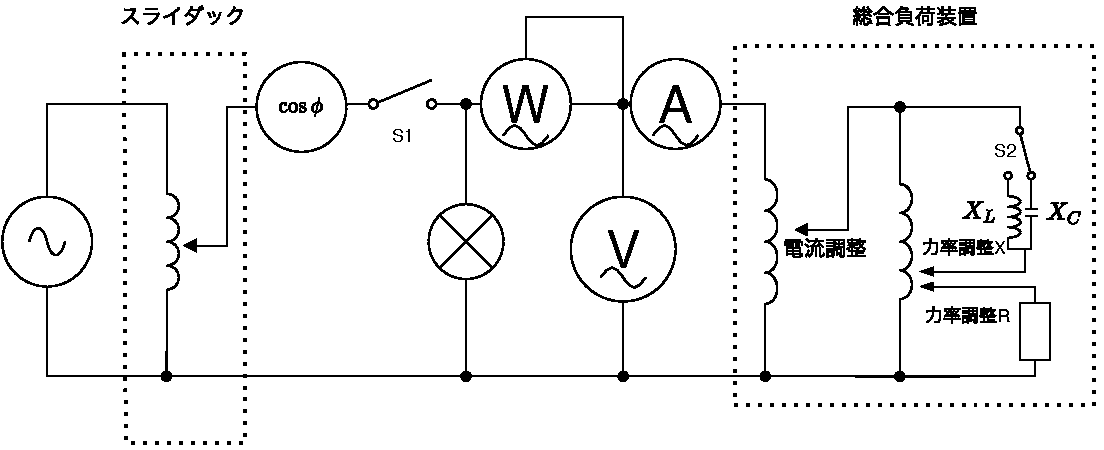
\includegraphics[scale=1]{./fig/circ.pdf}
	\caption{測定回路}
	\label{fig:circ}
\end{figure}
\item スイッチS1を開き,負荷の電流調節つまみをDEC方向いっぱいに回した.\footnote{DEC:decreaseの略で減らすの意.この処理は負荷に電流を加えないための初期設定}
\item スイッチS2を$X_{L}$側にし,リアクタンスとしてLを選択.\label{S2}
\item 力率を1に設定(負荷を$R=1.0, X=1.0$に設定)
\item S1を閉じ,商用電源の電圧(スライダック部)が$100\,\rm{V}$になるように調整し,総合負荷装置の電源ランプの点灯を確認した.
\item 電流計の読みが$1\,\rm{A}(\pm 0.1\,\rm{A})$となるようにSL1で電流を調整し,電力,力率,電圧,電流を計測.
\item 電流を$2\,\rm{A}$から$5\,\rm{A}$まで$1\,\rm{A}$刻みで同様の計測を実施.
\item 力率を以下のように設定し,上記の計測を繰り返した.
\begin{itemize}
	\item 力率0.8 ($R=0.8,\quad X=0.8$)
	\item 力率0.6 ($R=0.6,\quad X=0.6$)
	\item 力率0.4 ($R=0.4,\quad X=0.4$)
	\item 力率0.2 ($R=0.2,\quad X=0.2$)
\end{itemize}
\end{enumerate}
\item 電力計によるRC負荷の電力測定
\begin{enumerate}[(1)]
	\item \ref{RLhuka}を参考にし,\ref{S2}の部分でリアクタンスとしてCを選択した.(スイッチS2を$X_{C}$側に設定)
\end{enumerate}
\item 低力率用電力計による電力計測
\begin{enumerate}[(1)]
	\item \wfig{circ}において,電力計を低力率用のものに変更.
	\item 力率0.2 ($R=0.2,\quad X=0.2$)に設定し\ref{RLhuka}と同様の計測を行った.
\end{enumerate}
\end{enumerate}
\clearpage
\section{結果}
計測データの力率における負の値は進み位相を示している.
\begin{itemize}
	\item 負荷を$X_{L}$にした場合における各力率での計測データを\wtab{1data}から\wtab{0.2data}に示す.
	\item 負荷を$X_{C}$にした場合における各力率での計測データを\wtab{1data2}から\wtab{0.2data2}に示す.
	\item 負荷を$X_{L}$し,低力率計で計測したデータを\wtab{low0.2XL}に示す.
	\item 負荷を$X_{C}$し,低力率計で計測したデータを\wtab{low0.2XC}に示す.
\end{itemize}
	電流の増加とともに電力,皮相電力の増加および電圧の減少が見られる.また,計測力率$\cos \theta$が計算力率$\cos \theta '$より大きい場合が多い.
\begin{table}[h]
	\centering
	\caption{$X_{L}$,力率$1.0$での計測データ}
	\label{tab:1data}
\begin{tabular}{ccccccc}
	\hline
	電流[$\rm{A}$] & 電力$P_a[\rm{W}]$ & 電圧$V[\rm{V}]$ & 電流$I[\rm{A}]$ & 計測力率$\cos \theta$[\rm{-}]  & 計算力率$\cos \theta '$[ - ]  & 皮相電力$P_a[\rm{VA}]$ \\ \hline
	1      & 102.5   & 103.1   & 1.01  & 0.992 & 0.984 & 104.1   \\
	2      & 205.0   & 102.2   & 2.01  & 0.995 & 0.998 & 205.4   \\
	3      & 301.0   & 101.9   & 2.98  & 0.996 & 0.991 & 303.7   \\
	4      & 407.5   & 101.0   & 4.00  & 0.997 & 1.009 & 404.0   \\
	5      & 497.5   & 100.8   & 5.00  & 0.998 & 0.987 & 504.0     \\ \hline\\
\end{tabular}
	\caption{$X_{L}$,力率$0.8$での計測データ}
	\label{tab:0.8data}
\begin{tabular}{ccccccc}
	\hline
	電流[$\rm{A}$] & 電力$P_a[\rm{W}]$ & 電圧$V[\rm{V}]$ & 電流$I[\rm{A}]$ & 計測力率$\cos \theta$[ - ] & 計算力率$\cos \theta '$[ - ] & 皮相電力$P_a[\rm{VA}]$ \\ \hline
	1 & 59.0  & 104.3 & 1.00 & 0.830 & 0.566 & 104.3 \\
	2 & 160.0 & 104.0 & 1.95 & 0.817 & 0.789 & 202.8 \\
	3 & 242.5 & 102.9 & 3.01 & 0.800 & 0.783 & 309.7 \\
	4 & 322.5 & 102.3 & 4.04 & 0.798 & 0.780 & 413.3 \\
	5 & 395.0 & 101.9 & 5.01 & 0.798 & 0.774 & 510.5 \\ \hline\\
\end{tabular}
	\caption{$X_{L}$,力率$0.6$での計測データ}
	\label{tab:0.6data}
\begin{tabular}{ccccccc}
	\hline
	電流[$\rm{A}$] & 電力$P_a[\rm{W}]$ & 電圧$V[\rm{V}]$ & 電流$I[\rm{A}]$ & 計測力率$\cos \theta$[ - ] & 計算力率$\cos \theta '$[ - ] & 皮相電力$P_a[\rm{VA}]$ \\ \hline
	1 & 69.0  & 104.1 & 1.01 & 0.701 & 0.656 & 105.1 \\
	2 & 131.0 & 103.9 & 2.03 & 0.650 & 0.621 & 210.9 \\
	3 & 154.0 & 103.0 & 2.99 & 0.640 & 0.500 & 308.0 \\
	4 & 252.5 & 102.9 & 3.99 & 0.638 & 0.615 & 410.6 \\
	5 & 305.0 & 102.1 & 4.98 & 0.625 & 0.600 & 508.5 \\ \hline\\
\end{tabular}
	\caption{$X_{L}$,力率$0.4$での計測データ}
	\label{tab:0.4data}
\begin{tabular}{ccccccc}
	\hline
	電流[$\rm{A}$] & 電力$P_a[\rm{W}]$ & 電圧$V[\rm{V}]$ & 電流$I[\rm{A}]$ & 計測力率$\cos \theta$[ - ] & 計算力率$\cos \theta '$[ - ] & 皮相電力$P_a[\rm{VA}]$ \\ \hline
	1 & 55.0  & 104.7 & 1.00 & 0.570 & 0.525 & 104.7 \\
	2 & 97.5  & 104.0 & 2.04 & 0.500 & 0.460 & 212.2 \\
	3 & 136.0 & 103.8 & 3.00 & 0.478 & 0.437 & 311.4 \\
	4 & 179.0 & 103.1 & 4.01 & 0.470 & 0.433 & 413.4 \\
	5 & 217.0 & 103.0 & 5.01 & 0.460 & 0.421 & 516.0 \\ \hline\\
\end{tabular}
	\caption{$X_{L}$,力率$0.2$での計測データ}
	\label{tab:0.2data}
\begin{tabular}{ccccccc}
	\hline
	電流[$\rm{A}$] & 電力$P_a[\rm{W}]$ & 電圧$V[\rm{V}]$ & 電流$I[\rm{A}]$ & 計測力率$\cos \theta$[ - ] & 計算力率$\cos \theta '$[ - ] & 皮相電力$P_a[\rm{VA}]$ \\ \hline
	1 & 37.5  & 104.9 & 0.99 & 0.460 & 0.361 & 103.9 \\
	2 & 62.5  & 104.2 & 2.03 & 0.365 & 0.295 & 211.5 \\
	3 & 82.5  & 104.1 & 2.99 & 0.316 & 0.265 & 311.3 \\
	4 & 106.0 & 103.9 & 4.02 & 0.300 & 0.254 & 417.7 \\
	5 & 125.0 & 104.0 & 5.01 & 0.290 & 0.240 & 521.0 \\ \hline\\
\end{tabular}
\end{table}
\begin{table}[h]
\centering
	\caption{$X_{C}$,力率$1.0$での計測データ}
	\label{tab:1data2}
\begin{tabular}{ccccccc}
	\hline
	電流[$\rm{A}$] & 電力$P_a[\rm{W}]$ & 電圧$V[\rm{V}]$ & 電流$I[\rm{A}]$ & 計測力率$\cos \theta$[ - ] & 計算力率$\cos \theta '$[ - ] & 皮相電力$P_a[\rm{VA}]$ \\ \hline
	1 & 112.5 & 107.0 & 1.02 & 0.992 & 1.031 & 109.1 \\
	2 & 214.0 & 106.1 & 2.01 & 0.996 & 1.003 & 213.3 \\
	3 & 319.0 & 105.7 & 3.01 & 0.997 & 1.003 & 318.2 \\
	4 & 427.5 & 105.0 & 4.02 & 0.997 & 1.013 & 422.1 \\
	5 & 521.0 & 103.9 & 5.02 & 0.998 & 0.999 & 521.6 \\ \hline\\
\end{tabular}
	\caption{$X_{C}$,力率$0.8$での計測データ}
	\label{tab:0.8data2}
\begin{tabular}{ccccccc}
	\hline
	電流[$\rm{A}$] & 電力$P_a[\rm{W}]$ & 電圧$V[\rm{V}]$ & 電流$I[\rm{A}]$ & 計測力率$\cos \theta$[ - ] & 計算力率$\cos \theta '$[ - ] & 皮相電力$P_a[\rm{VA}]$ \\ \hline
	1 & 97.5  & 107.7 & 1.00 & -0.901 & 0.905 & 107.7 \\
	2 & 186.0 & 106.9 & 2.03 & -0.842 & 0.857 & 217.0 \\
	3 & 265.0 & 106.1 & 2.97 & -0.830 & 0.841 & 315.1 \\
	4 & 350.0 & 105.5 & 3.95 & -0.822 & 0.840 & 416.7 \\
	5 & 432.0 & 105.0 & 4.90 & -0.820 & 0.840 & 51.5  \\ \hline
\end{tabular}
	\caption{$X_{C}$,力率$0.6$での計測データ}
	\label{tab:0.6data2}
\begin{tabular}{ccccccc}
	\hline
	電流[$\rm{A}$] & 電力$P_a[\rm{W}]$ & 電圧$V[\rm{V}]$ & 電流$I[\rm{A}]$ & 計測力率$\cos \theta$[ - ] & 計算力率$\cos \theta '$[ - ] & 皮相電力$P_a[\rm{VA}]$ \\ \hline
	1 & 84.5  & 107.9 & 1.00 & -0.790 & 0.783 & 107.9 \\
	2 & 157.5 & 107.2 & 2.04 & -0.700 & 0.720 & 218.7 \\
	3 & 221.0 & 106.1 & 2.98 & -0.676 & 0.699 & 316.2 \\
	4 & 290.0 & 106.0 & 3.99 & -0.660 & 0.686 & 422.9 \\
	5 & 355.0 & 105.8 & 5.02 & -0.650 & 0.668 & 531.1 \\ \hline\\
\end{tabular}
	\caption{$X_{C}$,力率$0.4$での計測データ}
	\label{tab:0.4data2}
\begin{tabular}{ccccccc}
	\hline
	電流[$\rm{A}$] & 電力$P_a[\rm{W}]$ & 電圧$V[\rm{V}]$ & 電流$I[\rm{A}]$ & 計測力率$\cos \theta$[ - ] & 計算力率$\cos \theta '$[ - ] & 皮相電力$P_a[\rm{VA}]$ \\ \hline
	1 & 69.0  & 107.9 & 1.01 & -0.640 & 0.633 & 109.0 \\
	2 & 116.0 & 107.5 & 2.02 & -0.520 & 0.534 & 217.2 \\
	3 & 161.0 & 107.0 & 2.99 & -0.480 & 0.503 & 319.9 \\
	4 & 211.0 & 106.9 & 3.98 & -0.466 & 0.496 & 425.5 \\
	5 & 305.0 & 106.2 & 5.03 & -0.458 & 0.571 & 534.2 \\ \hline\\
\end{tabular}
	\caption{$X_{C}$,力率$0.2$での計測データ}
	\label{tab:0.2data2}
\begin{tabular}{ccccccc}
\hline
電流[$\rm{A}$] & 電力$P_a[\rm{W}]$ & 電圧$V[\rm{V}]$ & 電流$I[\rm{A}]$ & 計測力率$\cos \theta$[ - ] & 計算力率$\cos \theta '$[ - ] & 皮相電力$P_a[\rm{VA}]$ \\ \hline
1 & 45.0  & 108.1 & 0.99 & -0.480 & 0.420 & 107.0 \\
2 & 70.0  & 107.9 & 2.01 & -0.320 & 0.323 & 216.9 \\
3 & 94.0  & 107.8 & 3.00 & -0.280 & 0.291 & 323.4 \\
4 & 120.0 & 107.7 & 4.08 & -0.260 & 0.273 & 439.4 \\
5 & 144.0 & 107.1 & 5.00 & -0.240 & 0.269 & 535.5 \\ \hline
\end{tabular}
\end{table}
\begin{table}[h]
\centering
\caption{低力率計を用いた$X_{L}$,力率$0.2$での計測データ}
\label{tab:low0.2XL}
\begin{tabular}{ccccccc}
	\hline
	電流[$\rm{A}$] & 電力$P_a[\rm{W}]$ & 電圧$V[\rm{V}]$ & 電流$I[\rm{A}]$ & 計測力率$\cos \theta$[ - ] & 計算力率$\cos \theta '$[ - ] & 皮相電力$P_a[\rm{VA}]$ \\ \hline
	1 & 39.0  & 106.8 & 1.00 & 0.462 & 0.365 & 106.8 \\
	2 & 63.8  & 106.8 & 2.00 & 0.360 & 0.299 & 213.6 \\
	3 & 84.0  & 106.5 & 3.05 & 0.308 & 0.259 & 324.8 \\
	4 & 106.0 & 106.1 & 3.98 & 0.300 & 0.251 & 422.3 \\ \hline\\
\end{tabular}
\caption{低力率計を用いた$X_{C}$,力率$0.2$での計測データ}
\label{tab:low0.2XC}
\begin{tabular}{ccccccc}
\hline
電流[$\rm{A}$] & 電力$P_a[\rm{W}]$ & 電圧$V[\rm{V}]$ & 電流$I[\rm{A}]$ & 計測力率$\cos \theta$[ - ] & 計算力率$\cos \theta '$[ - ] & 皮相電力$P_a[\rm{VA}]$ \\ \hline
1 & 46.5  & 106.9 & 1.00 & -0.484 & 0.435 & 106.9 \\
2 & 71.5  & 106.3 & 2.01 & -0.340 & 0.335 & 213.7 \\
3 & 95.8  & 106.0 & 2.99 & -0.300 & 0.302 & 316.9 \\
4 & 119.5 & 105.9 & 4.01 & -0.280 & 0.281 & 424.7 \\ \hline
\end{tabular}
\end{table}


\section{考察}
\section{結論}

\newpage
\printbibliography[title=参考文献]

\end{document}